% $Id%

\newpage
\hypertarget{appendix-start}{}\label{s:appendix-start}


\section{Appendix}

\hyperlink{appendix-menutree}{(Appendix A: CrypTool Menu Tree)}

\hyperlink{appendix-authors}{(Appendix B: CrypTool Script Authors)}

\hyperlink{appendix-movies}{(Appendix C: Movies and Literature with Relation to Cryptography)} 



%\pagebreak
\newpage
\enlargethispage{1cm}
\subsection{CrypTool Menus}
\hypertarget{appendix-menutree}{}\label{s:appendix-menutree}

This appendix contains the complete menu tree of CrypTool\index{CrypTool} version 1.3.10. 

Which menu items are active (that is not greyed), depends on the type 
of the currently active document window.
The brute-force analysis\index{Attack!brute-force} for DES e.~g. is only
available, if the active window is opened in the hexadecimal view. 
On the other hand the menu item
``Generate Random Numbers\dots'' is always available.

The following types of documents exist in CrypTool:
\begin{center}
\begin{tabular}{rl}
\bf Code letter & \bf Type of document \\
A & ASC\\
T & Text\\
H & Hexadecimal\\
P & Plot\\
\end{tabular}
\end{center}

%\nobreak
\clearpage
\begin{figure}[hb]
\begin{center}
\vspace{-30pt}
%\frame{
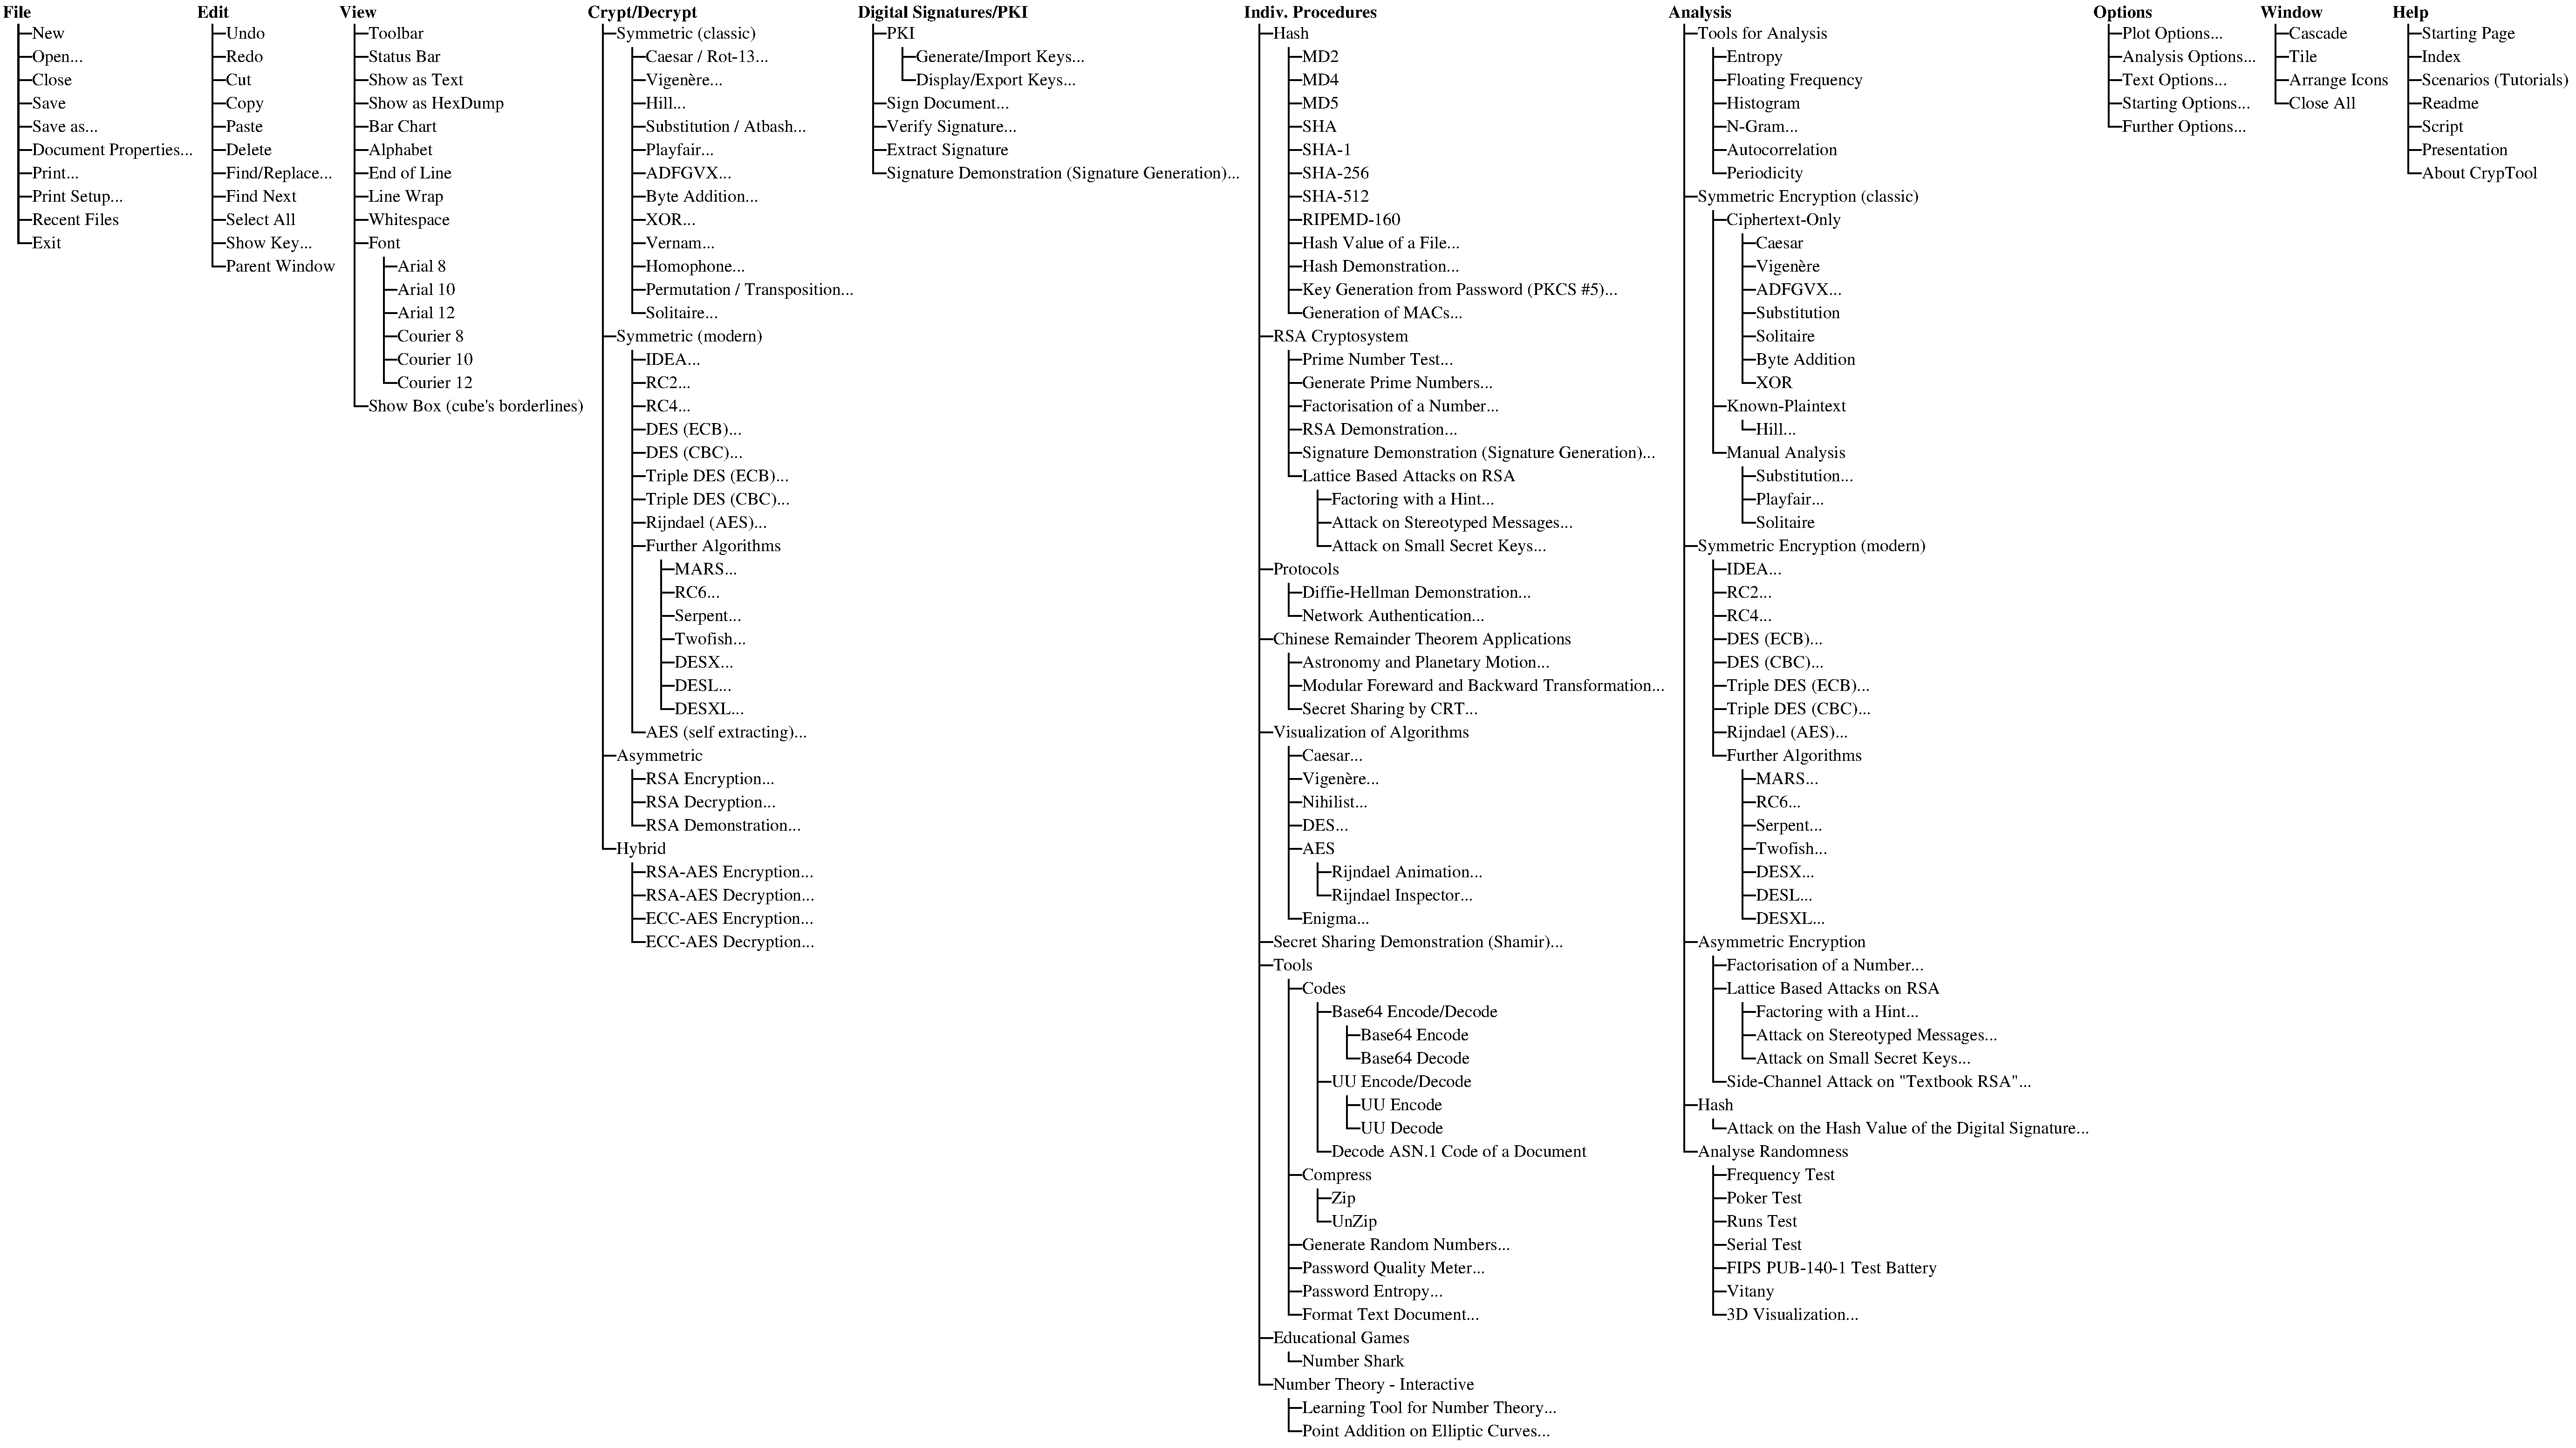
\includegraphics[scale=0.75, angle=270, viewport=14 72 835 590]{figures/cryptool-menu-en}
%viewport=rand-links? rand-unten breite hoehe? [bezogen auf querformat]
%}
\caption{Complete overview of the CrypTool menu tree} 
\label{menuoverview}
\end{center}
\end{figure}
\clearpage

